\documentclass{article}
\usepackage{graphicx}
\usepackage{hyperref}
\usepackage{geometry}
\geometry{a4paper, margin=1in}

\title{Progress Report: FRB Host Galaxy Analysis}
\author{GitHub Copilot}
\date{\today}

\begin{document}

\maketitle

\section{Photutils Inclination Analysis}
Minimal comparison between \texttt{photutils}, GALFIT, and SDSS inclinations.

\begin{figure}[h!]
    \centering
    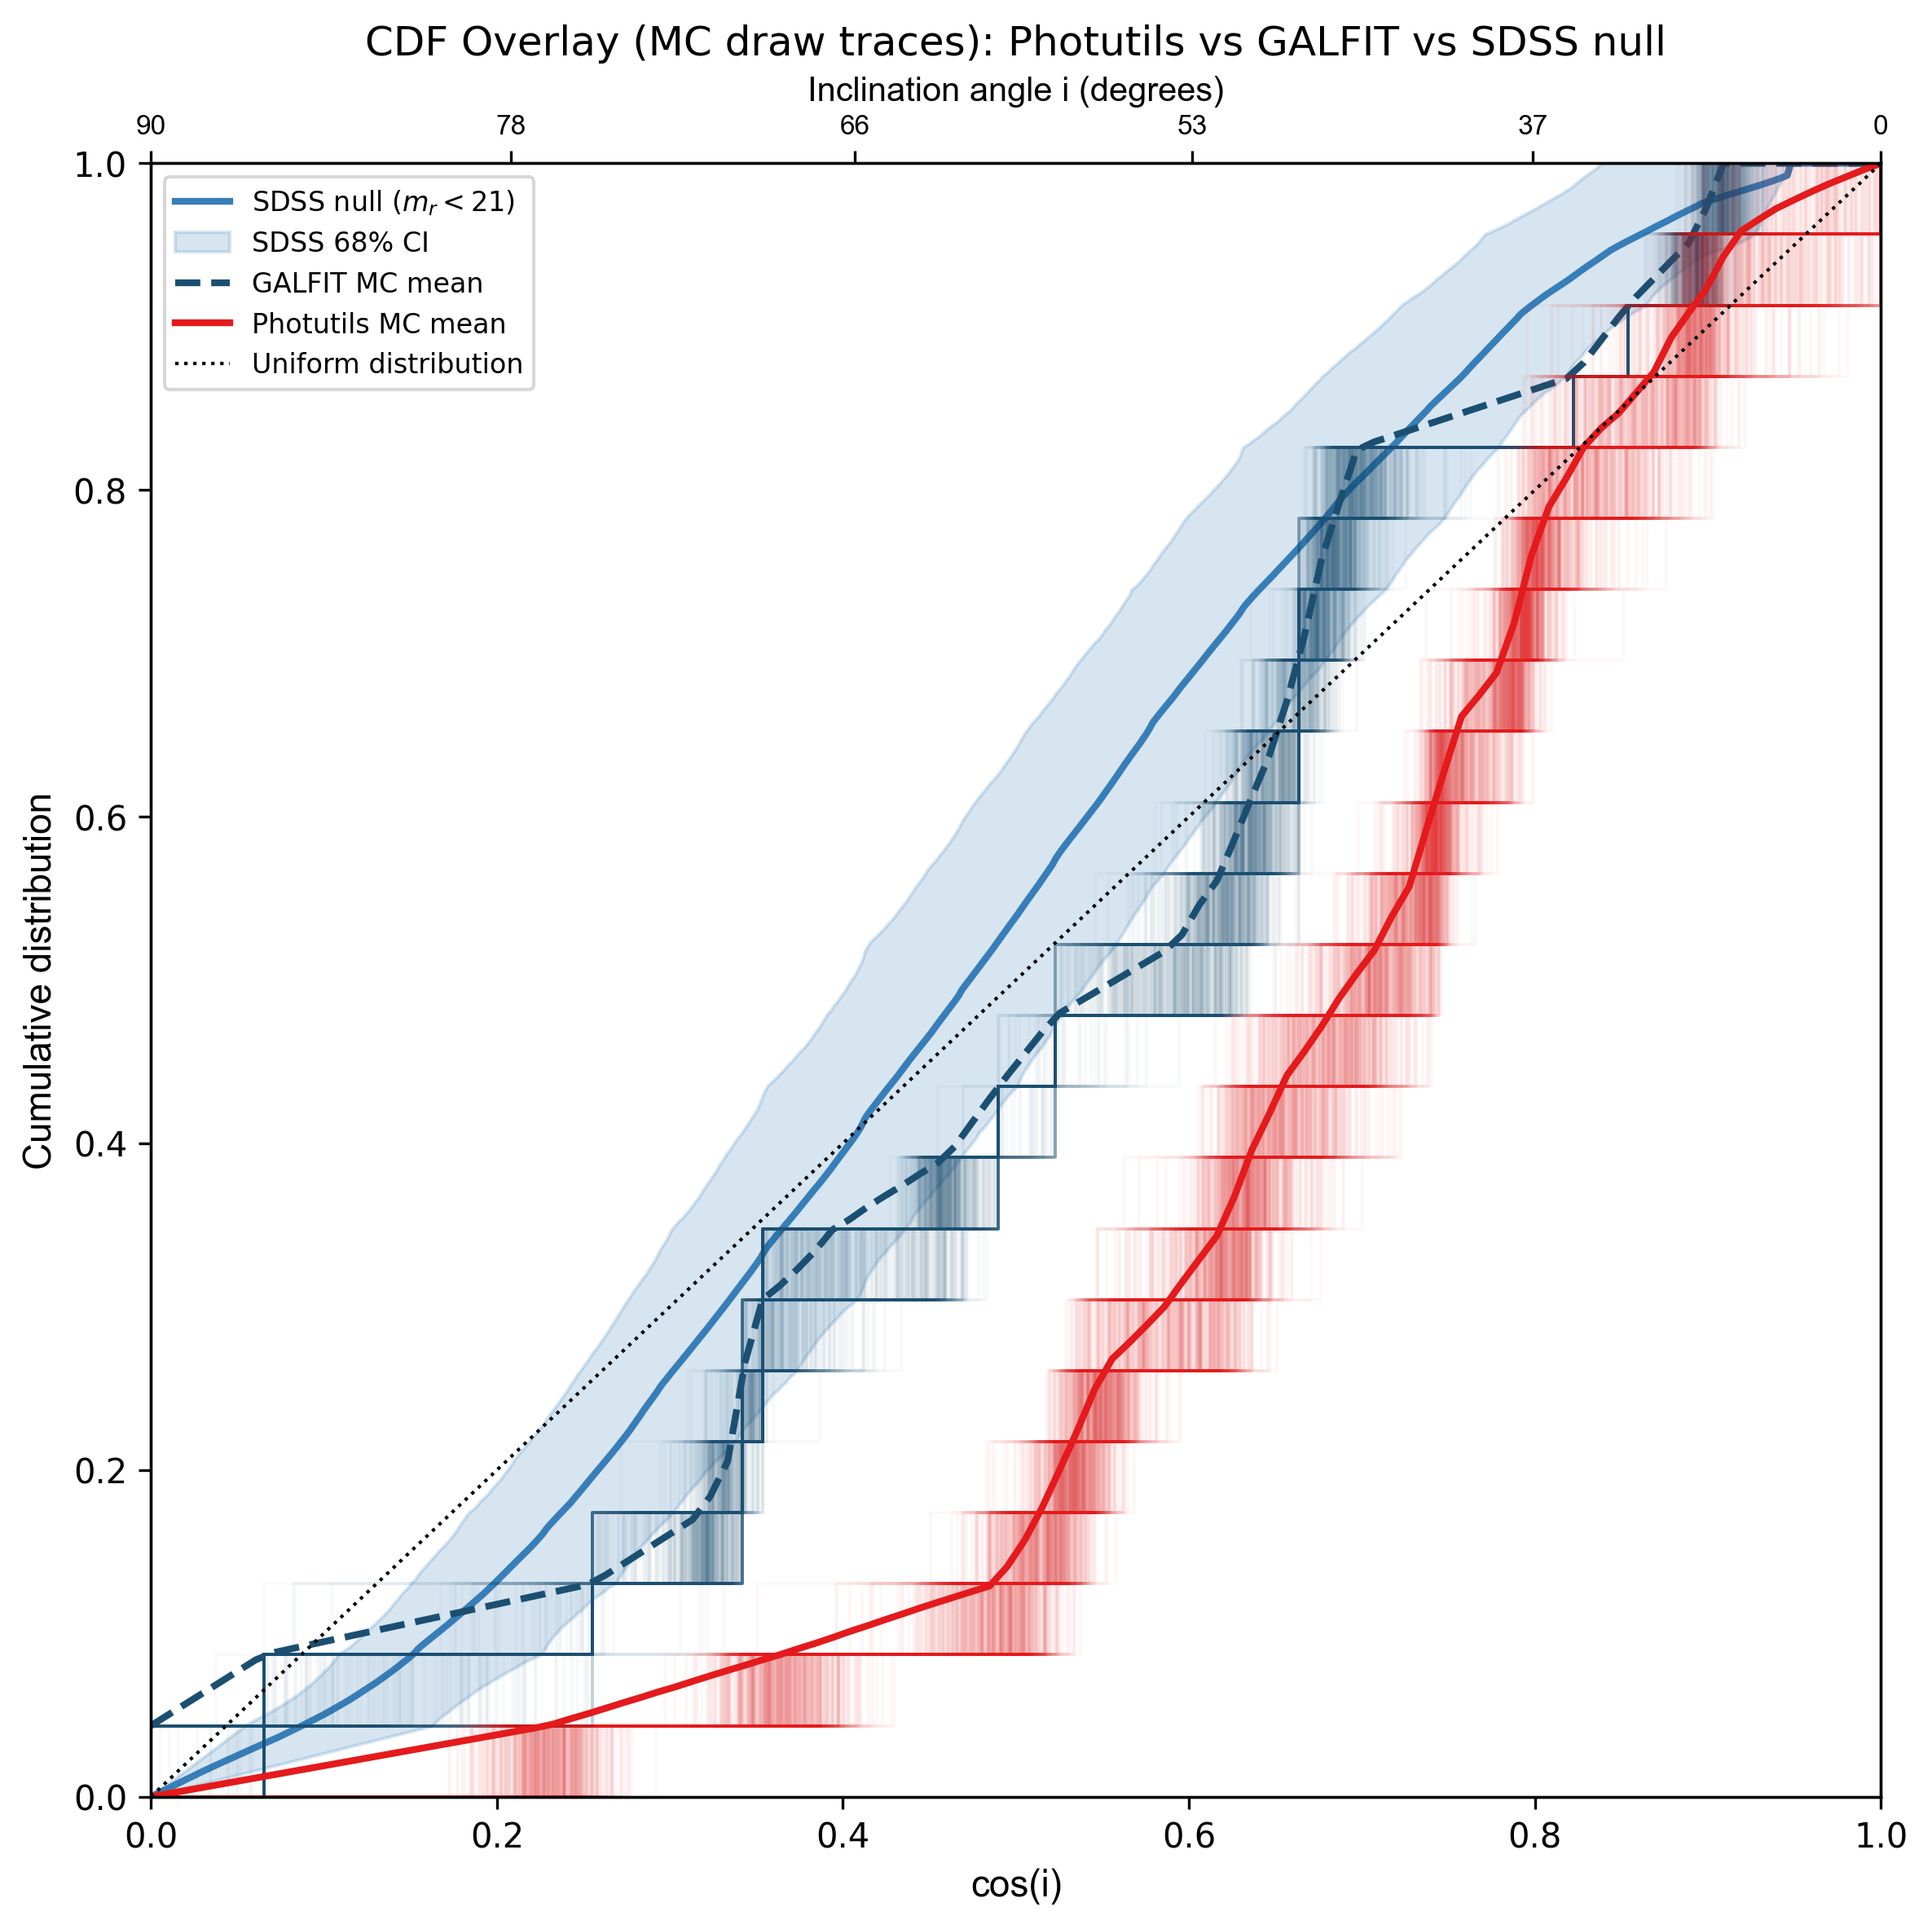
\includegraphics[width=0.8\textwidth]{images/photutils_vs_galfit_vs_sdss_nopsf_spaghetti.png}
    \caption{GALFIT and Photutils inclination comparisons against SDSS, including Monte Carlo uncertainty tracks.}
    \label{fig:mc_comparison}
\end{figure}

\begin{figure}[h!]
    \centering
    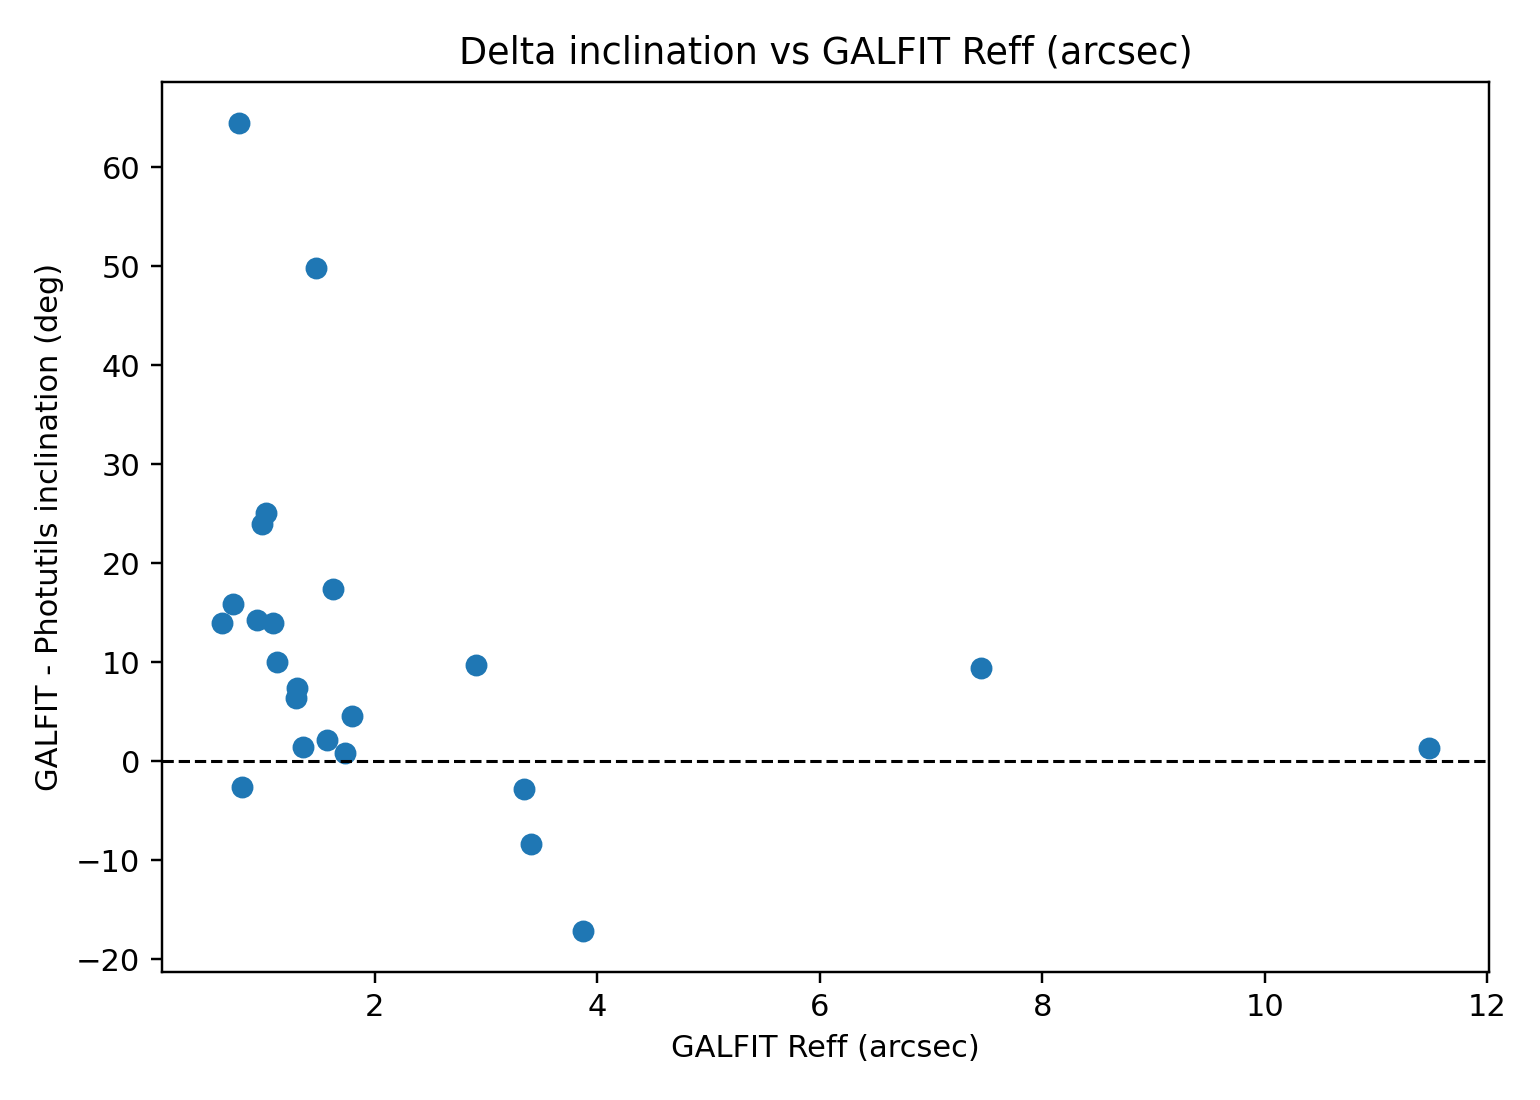
\includegraphics[width=0.8\textwidth]{images/delta_inc_galfit_minus_photutils_vs_galfit_reff_arcsec.png}
    \caption{Difference in inclination (GALFIT - Photutils) vs. GALFIT effective radius in arcseconds.}
    \label{fig:delta_inc_reff}
\end{figure}

\begin{figure}[h!]
    \centering
    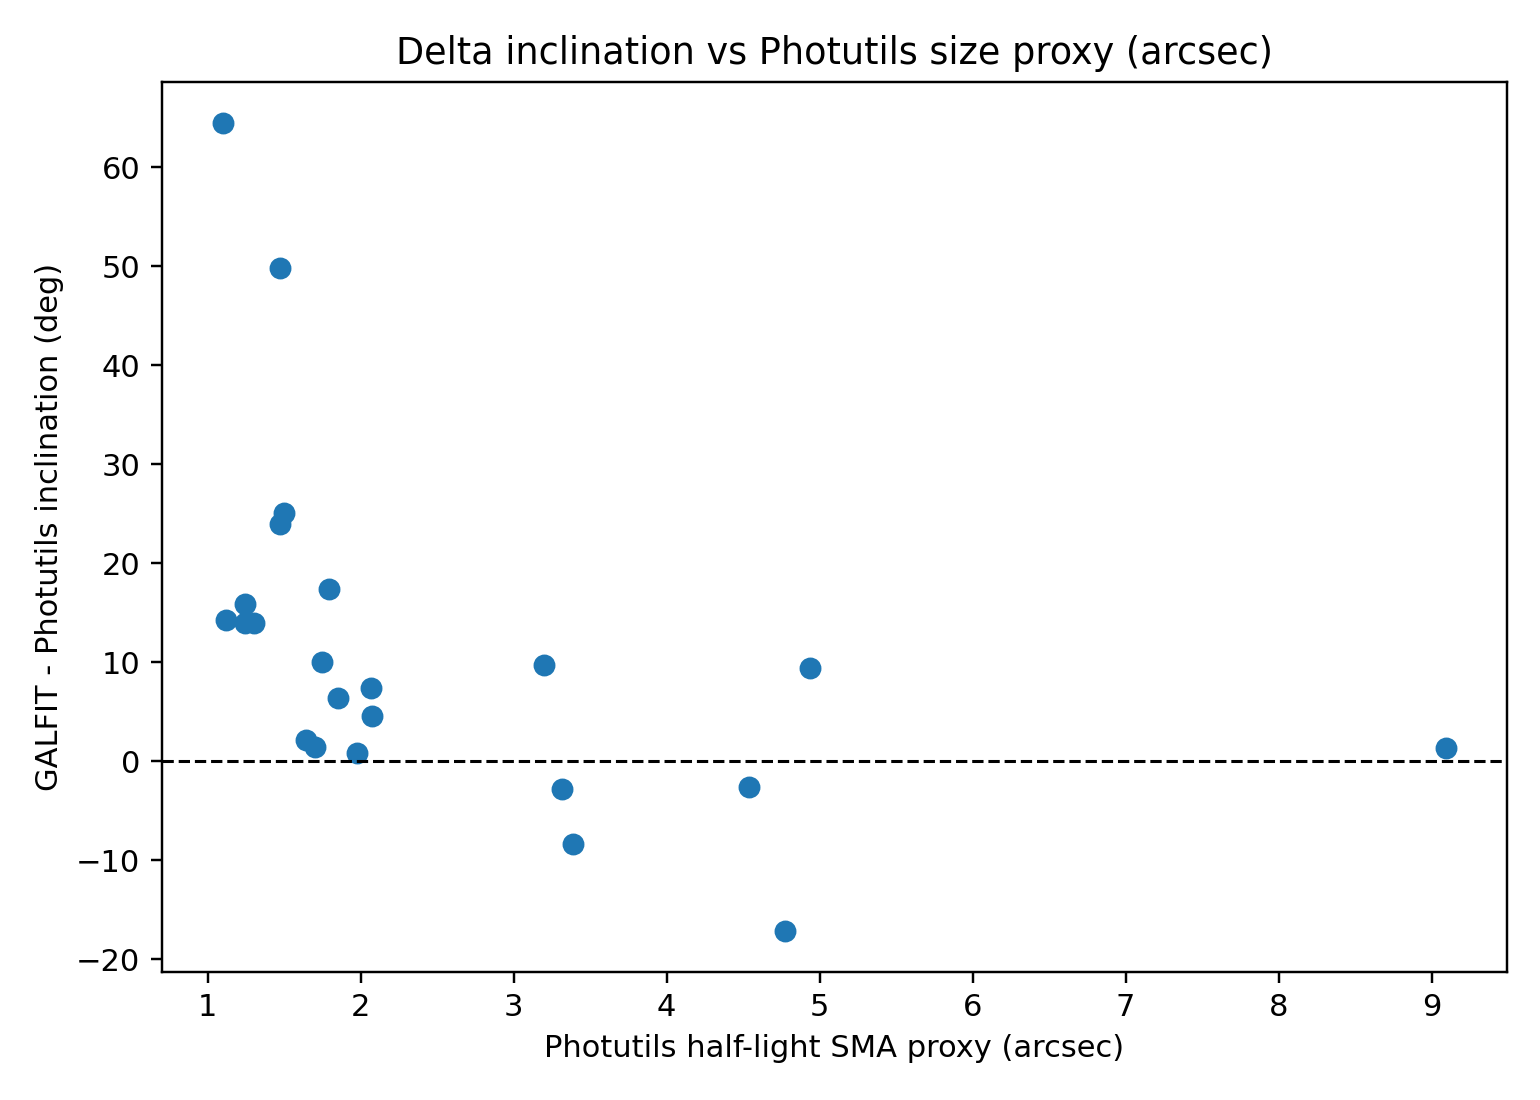
\includegraphics[width=0.8\textwidth]{images/delta_inc_galfit_minus_photutils_vs_photutils_sma_proxy_arcsec.png}
    \caption{Difference in inclination (GALFIT - Photutils) vs. Photutils semi-major axis proxy in arcseconds.}
    \label{fig:delta_inc_sma}
\end{figure}

\clearpage

\section{Legacy Survey vs. GALFIT Comparison}
\noindent Even as \(n\) changes massively, \(R_{\mathrm{eff}}\) remains nearly the same in Legacy Survey fits; with model and residual images looking so similar, the fitting behavior is confusing.

\input{legacy_vs_galfit_selected_fields_all_rows_table.tex}

\begin{figure}[h!]
    \centering
    
\includegraphics[width=\textwidth]{images/panel_top_delta_i_no_rex_13_full.png}
    \caption{Top 13 inclination deviations (excluding REX), with FRB names labeled above each IMR row.}
    \label{fig:imr_panel}
\end{figure}

\clearpage

\section{Potential FRB Data Sources}
Currently exploring the sources -

\begin{itemize}
    \item \href{https://www.frb-hosts.org/}{frb-hosts.org}: 9 FRBs, 5 unique
    \item \href{https://github.com/FRBs/FRB/blob/main/docs/database.rst}{FRBs/FRB database.rst}: not explored yet
    \item \href{https://www.chime-frb.ca/catalog}{CHIME/FRB catalog}: unsure whether these are localized
    \item \href{https://iopscience.iop.org/article/10.3847/1538-4357/abb6fb/pdf}{ApJ 10.3847/1538-4357/abb6fb}: 13 with 5 unique
    \item \href{https://iopscience.iop.org/article/10.3847/1538-4357/ace5aa/pdf}{ApJ 10.3847/1538-4357/ace5aa}: 23 with 3 new
    \item \href{https://github.com/krittisharma/frb_host_sharma2024}{frb\_host\_sharma2024}: not explored yet
\end{itemize}

\noindent Total identified so far: 13 new unique FRBs.

\end{document}
